\def\year{2019}
%File: formatting-instruction.tex
\documentclass[letterpaper]{article}
\usepackage{aaai19}
\usepackage{paralist}
\usepackage{graphicx, color}
%\usepackage{subfigure}
\usepackage{booktabs}
%\usepackage{caption}
%\usepackage{subcaption}
\usepackage{paralist}
\usepackage{amssymb, amsmath, amsthm, amsfonts} 
\newtheorem{myProb}{Problem}
%\usepackage[ruled]{algorithm2e}
%\usepackage[colorinlistoftodos]{todonotes}
%\usepackage{todonotes}
%\usepackage{Algorithmic}
% include custom modifications
%\usepackage{_style/review}
% \usepackage{subfigure}
%\newcommand{\nonl}{\renewcommand{\nl}{\let\nl\oldnl}}
%\newcommand{\RNum}[1]{\uppercase\expandafter{\romannumeral #1\relax}}
%\usepackage[ruled]{algorithm2e}
\graphicspath{{./Figures/}}
%\documentclass{llncs}
%\usepackage[ruled]{algorithm2e}
%\usepackage{Algorithmic}
%\usepackage{times}
\usepackage{multirow}
\usepackage{subfig}
\usepackage{microtype}
%\usepackage{url}
\usepackage{balance}
\usepackage{graphicx, color}
%\usepackage{subfigure}
%\usepackage{wrapfig}
%\usepackage{paralist}
\usepackage[draft]{hyperref}
%\let\proof\relax 
%\let\endproof\relax
\newtheorem{mydef}{Definition}
\usepackage{mwe}

%\usepackage{amssymb, amsmath,amsthm} 
\usepackage{relsize}
\usepackage{pdflscape}
\usepackage{comment}
\usepackage[ruled]{algorithm2e}
\newtheorem{mylemm}{Lemma}
\newcommand{\mypar}[1]{\smallskip\noindent\textbf{#1.}}
\setcounter{secnumdepth}{3}
\newcommand{\todo}[1]{\textcolor{red}{\bf {#1}}}
%\usepackage[document]{ragged2e}
\renewcommand{\sectionautorefname}{Section}
\renewcommand{\subsectionautorefname}{Section}
\newtheorem{mycor}{Corollary}
\newtheorem{mythm}{Theorem}
\newtheorem{myprop}{Proposition}
%
% paper title
% Titles are generally capitalized except for words such as a, an, and, as,
% at, but, by, for, in, nor, of, on, or, the, to and up, which are usually
% not capitalized unless they are the first or last word of the title.
% Linebreaks \\ can be used within to get better formatting as desired.
% Do not put math or special symbols in the title.
\begin{document}
	
\title{Learning Scheduling Models from Event Data}



% author names and affiliations
% use a multiple column layout for up to three different
% affiliations
%\author{\authorblockN{Arik Senderovich, Kyle E.C. Booth,
%		J. Christopher Beck} \authorblockA{Argh}}
\author{removed for review\vspace{3.4em}}
%\author{\IEEEauthorblockN{Arik Senderovich\IEEEauthorrefmark{1},
%		Matthias Weidlich\IEEEauthorrefmark{2}, and
%		Avigdor Gal\IEEEauthorrefmark{1}}
%	\IEEEauthorblockA{\IEEEauthorrefmark{1}Technion -- Israel Institute of 
%	Technology\\ 
%						Emails: sariks,avigal@technion.ac.il}
%	\IEEEauthorblockA{\IEEEauthorrefmark{2}Humboldt University zu Berlin\\
%			Email: matthias.weidlich@hu-berlin.de}}

\maketitle

\begin{abstract}
Solving scheduling problems
requires two main ingredients: a model 
that captures 
the essence of the underlying system and an algorithm that 
provides optimal solutions based on the model.
Constraint programming (CP) is a well-established
paradigm for modeling and solving deterministic
scheduling problems.  
It has been well-recognized that creating a suitable CP model is knowledge intensive 
task even when the underlying system is 
well-understood.  
In this work, we
aim at 
automating
the process of 
modeling scheduling problems
by learning CP models from event data.
To this end, 
we introduce
a novel methodology 
that combines process mining, 
timed Petri nets and CP.
As a first step, the approach
mines
timed Petri nets (TPNs) from event logs
that contain
executions of past schedules including
information on activities, timestamps and resources.
For the second step, 
we define a specialized TPN type,
namely the seize-delay-release net with 
resources (SDRR net),
which can be mapped into CP models. 
We provide a correct and complete algorithm
for detecting whether a TPN is an SDRR net.
Furthermore, we show a
mapping from SDRR nets into CP models.
Our approach provides an end-to-end solution
to model learning, going from 
event logs to model-based optimal schedules
without human intervention. 
To demonstrate the usefulness 
of the methodology we conduct
a series of experiments in which we
learn scheduling models from
two types of data: (1) event logs generated from 
job-shop scheduling benchmarks and (2) real-world event
logs that come from an outpatient hospital. 

\end{abstract}



% no keywords





% For peer review papers, you can put extra information on the cover
% page as needed:
% \ifCLASSOPTIONpeerreview
% \begin{center} \bfseries EDICS Category: 3-BBND \end{center}
% \fi
%
% For peerreview papers, this IEEEtran command inserts a page break and
% creates the second title. It will be ignored for other modes.
%\IEEEpeerreviewmaketitle



\section{Introduction}
\label{sec:introduction}

Modern scheduling algorithms 
successfully solve
problems with thousands of
activities, complex temporal constraints,
and scarce resources. The main two prerequisites to 
solving scheduling problems are 
(1) a mathematical
model that describes the system
and (2) an algorithm that 
solves the problem based on the aforementioned model.

In deterministic scheduling,
Constraint Programming (CP) has been shown to 
be extremely effective in solving a wide range
of problems~\cite[Chapter 6]{Baptiste:2001},~\cite{lallouet2010learning}.  
However, creating CP
models  
often requires 
a high level
of expertise, as one must specify 
suitable variables, constraints and objective
functions that 
correspond to the underlying real-world problem~\cite{lallouet2010learning}. 

In this work, we address the challenge
of automating 
the process of modeling scheduling problems
by learning CP models from data. Previous works
that learn CP models 
assume that the data is tightly coupled 
with the CP formulation. 
For example, when learning from positive
examples only, the data at hand must contain
variables as they appear in CP models~\cite{beldiceanu2012model}. In other works,
it is assumed that
the data must include 
both positive and negative labels for
assignments that satisfy 
or violate constraints, respectively~\cite{lallouet2010learning}. 

In practice, for many real-world problems
existing data recordings do not 
relate to the CP formalism (e.g., does
not include variables). Instead, the data comes in the form of 
event logs,
which are logs that contain the activities that 
were executed, along with their 
start and completion times,
and 
information on resource consumptions~\cite[Chapter 4]{AalstBook}.
In this work, we address the challenge of learning 
scheduling models 
automatically from event logs without humans intervention.
 \begin{figure*}[t!]
	\centering
	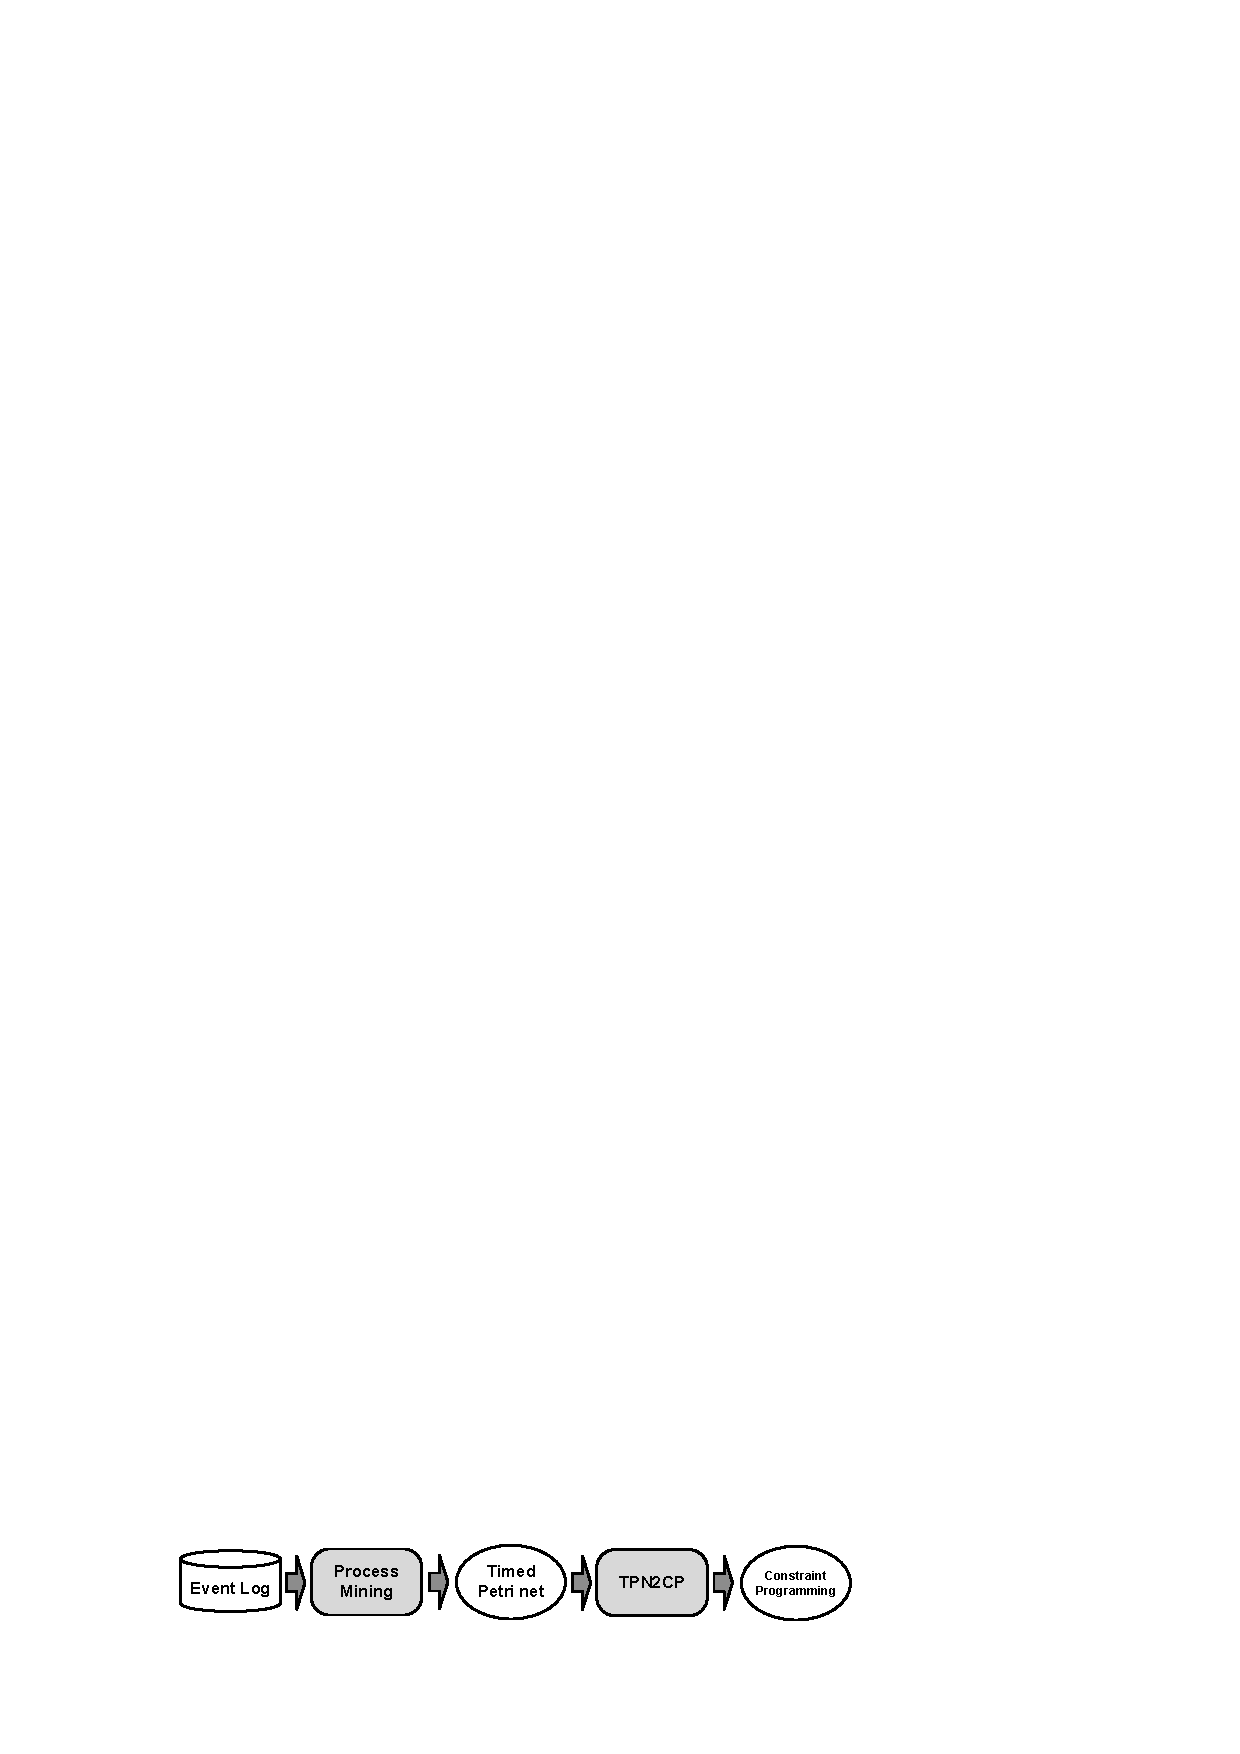
\includegraphics[scale= 0.8]{Approach.pdf}
	\vspace{-0.5em}
	\caption{Our solution to learning scheduling models.}
	\label{fig:overview}
	%  \vspace{-0.8em}
\end{figure*}
Figure~\ref{fig:overview} presents an overview of our approach.
As our first step, we use existing techniques from process mining,
a rapidly developing
research field that aims at learning models
of the underlying process 
from event logs~\cite{AalstBook}. Specifically,
we apply a model learning method
that considers scheduled processes and their execution data~\cite{SenderovichRGMM15}. The result of the 
process mining step is a 
timed Petri net (TPN), a well-known formalism
for modeling dynamic schedule-driven systems~\cite{van1996petri}.
Since the TPN is highly expressive and 
captures synchronization, resource consumption, and temporal constraints, it cannot be used efficiently 
for scheduling the system that it models~\cite{van1996petri}. 
Therefore, in the next step we transform the learned 
TPN into a CP model. 
However, due to differences in the expressive power
of the two formalisms (TPN and CP), we must 
restrict the TPN to a family of models that can be 
transformed into CP formulations. To this end, we define a 
new type of TPNs, namely Seize-Delay-Release nets with resources (SDRR nets). We show a correct and complete algorithm that given a TPN verifies that it is an SDRR net. Subsequently, if the 
TPN is an SDRR net, we provide a 
correct and complete mapping of the SDRR net into a CP model,
thus completing our solution to learning CP models from event data. 
 


The main contribution of our work is threefold: \begin{itemize}
\item We provide an data-to-model solution that learns scheduling models from event logs.
\item We introduce a specialized type of timed Petri nets, namely
the SDRR nets, which enables a TPN to CP transformation. 
\item We show a correct and complete algorithm for verifying
that a TPN is an SDRR net
and provide a mapping of SDRR nets into CP models.

\end{itemize}

To demonstrate the usefulness of our approach,
we provide a two-part experimental evaluation.
In the first part, we learn 
models of job-shop scheduling
benchmarks using 
synthetically generated data. In the second part of the evaluation,
we learn scheduling models from real-world data
coming from a large outpatient cancel hospital in the United States. 
Given the data, our algorithms generate
the underlying appointment scheduling problem 
that we consequently solve 
using constraint programming.

 

\section{Background}
\label{sec:preliminaries}

In this section we present 
the preliminaries to 
our approach. Firstly, we define timed Petri nets, a special case of 
stochastic Petri nets as defined in ~\cite[Chapter 2]{haas2002stochastic},
having 
deterministic activity durations and routing. 
Secondly, we define our data model in the form of events logs and 
briefly outline existing approaches
for learning TPN models from event logs. We conclude the section with a
definition of a general family of scheduling problems,
namely \emph{basic scheduling problems} (BSP).

\subsection{Timed Petri Nets}

Petri nets are procedural 
models 
for analyzing discrete-event dynamic systems that exhibit 
parallelism, synchronization and resource consumption.
Formally, a timed Petri net (TPN) is defined as follows: \begin{mydef} [Timed Petri net (TPN); TPN System] \label{def:tpn}
	A timed petri net $\mathcal{N}$ is a 
	tuple $\mathcal{N} = \langle E, E',P, F, \tau\rangle$ with,
	\begin{itemize}
		\item $E$ being a finite set of transitions with $E' \subseteq E$ being a (possibly empty) set of timed transitions, 
		\item $P$ being a finite set of places,
		\item $F \subseteq E \times P \cup P \times E $ being the flow relation of the Petri net, and, 
		\item $\tau \in (E' \rightarrow \mathcal{T})$ being a function that maps deterministic durations
		to timed transitions;
	\end{itemize} 
\end{mydef} A TPN is fully characterized as 
a pair $(\mathcal{N}, m_0)$ with $\mathcal{N}$ being the net and $m_0: P \rightarrow \mathbb{N}$ being an initial marking of the net, which is a 
function that maps each place to the number of tokens that it contains. We use Figure X to demonstrate a TPN and its dynamic behavior. In the figure, we observe two jobs waiting in the queue place.... \todo{Insert simple (not too simple) TPN example here to explain the dynamics} We denote $\bullet p$ ($\bullet e$) the set of
transitions (places) that precede a place $p$ (a transition $e$), and by $p \bullet$ the 
set of transitions (places) that succeed a place $p$ (a transition $e$). 
Furthermore, we define $F_P$ to be the 
set of incoming and outgoing flows the 
corresponds to a set of places $P$, i.e.,
$F_P = \{(x,y) \in F \ |\ x \in P \ \lor \ y \in P \}$.


For example,
in Figure X $\bullet p_3$... \todo{complete here} 

%
%The set of input (output) places is 
%denoted $P_{input} \subseteq P$ ($P_{output} \subseteq P$), such that $\forall p \in P_{input} \ (\bullet p = \emptyset)$ ($\forall p \in P_{output} \ (p\bullet = \emptyset))$). We shall assume that $|P_{input}|>0$ and $|P_{output}|>0$ (TPN has at least a single input and a single output). Also, we assume that $|e\bullet|>1$ and $|\bullet e|>1$ (every transition is followed and preceded by at least one place). Finally, the structural part of the TPN ($\mathcal{N}$) can be represented by a graph, $\mathcal{G}(\mathcal{N}) = (P \cup T, F)$, with $P \cup T$ being its nodes, and $F$ being its edges.
 
TPNs were previously applied
to model scheduling problems~\cite{van1996petri,lee1994scheduling}. 
However, they provide an inefficient solution platform for solving scheduling
problems,
since TPNs require a 
global search over 
the entire state-space
of the underlying problem~\cite{lee1994scheduling}. 
Therefore, 
previous literature on scheduling with Petri nets mostly
focuses on heuristic solutions~\cite{lee1994scheduling}.

\subsection{Mining Timed Petri nets from Event Logs}

Process mining is a rapidly evolving research field 
that is centered around developing methodologies
for learning models from data~\cite{AalstBook}.
The assumption is that the execution of processes
is recorded into event logs, which can in turn be employed 
to learn models of the underlying system
(e.g., in the form of a Petri net). The learning
task is typically assumed to be unsupervised, since 
the learned model cannot be validated against ground truth. 

To define process learning, we must first give an overview of
our data model, namely the event log. 
Let $\mathcal{E}$ be the universe of events
with $e \in \mathcal{E}$ having attributes $e.j$ for 
job identifier, $e.s$ for start of operation 
timestamp, $e.c$ for completion of operation timestamp, 
$e.R$ for resource and $e.A$ for event label (e.g., operation 3 start, operation 5 complete, operation 7 start). 
An event log $L$ is a subset of $\mathcal{E}$. 
Figure Y presents an excerpt from a real-world event log
of an outpatient cancer hospital. Furthermore,
we let $\psi(L,M) \in [0,1]$ be a learning
quality function that given
an event log $L$ and a TPN $M$ evaluates the model 
with $0$ ($1$) indicating low (high) quality model
with respect to the log. 

The task of a process learning function $\gamma$ that maps 
an event log $L$ onto a Petri net model $M$ (in our case a TPN)
such that $\psi(L,\gamma(L))$ is minimized~\cite{AalstBook}. 
The measure $\psi$ measures the distance
between model and log indirectly,
since we do not assume to have labeled pairs of logs and models.
Many process learning algorithms were proposed in the past. See Chapter X
in~\cite{AalstBook} for a survey.

In this work, we learn TPNs using the
approach developed 
for scheduled processes~\cite{DBLP:conf/bpm/SenderovichRGMM15}.
Specifically, the method in~\cite{DBLP:conf/bpm/SenderovichRGMM15} learns
the various components of the TPN, 
while guaranteeing maximal quality value, assuming
that the event log was generated by 
a process that followed a pre-defined schedule.
\todo{Should we add more details here? no options between operations and loops are allowed}
 






%
%\section{Solution Overview}
%\label{sec:solution}




In this section, we provide our end-to-end 
solution for learning scheduling models from data, as illustrated in Figure~\ref{fig:overview}. 
Given an event log, we apply a process mining method from~\cite{} 
to discover a timed Petri net, which represents
the underlying system. 



\section{Schedule-Driven Petri Nets}
In this section, we provide
our approach to solving the 
schedule learning problem. 
We assume that a TPN
is learned from event data using
existing approaches, e.g., via the approach presented 
in~\cite{DBLP:conf/bpm/SenderovichRGMM15}.
\todo{we actually make a modification that enables 
	that some of the activities can be performed by alternating sets of resources}.

\subsection{Seize-Delay-Release Nets}

The transformation of a learned TPN into a BSP,
is based on the notion 
of Seize-Delay-Release nets with resources (SDRR nets). 

To define SDRR nets, 
we first consider seize-delay-release constructs (SDCs), 
which are 
TPNs that consist of the following three components:
(1) two transitions: one immediate transition that seizes a token and 
one timed transition that releases the token after a delay, (2) a place where the
token is delayed, and (3) two flows that connect the two transitions to the delay place. 
Formally,
\begin{mydef} [Seize-Delay Construct (SDC)] \label{def:sdc}
	An SDC is a timed Petri net, 
	$\mathcal{S} = \langle E, E' , P , F, \tau \rangle)\rangle$, such that 
	\begin{itemize}
		\item The set $E = \{ e_{seize}, e_{release} \}$ contains two transitions (seize and delay), 
		\item The set $E' = \{e_{release}\}$ is the timed delay transition, 
		\item The set $P = \{p_{delay}\}$ is a single delay place, and,
		\item The flow is $F = \{ (e_{seize}, p_{delay}), (p_{delay}, e_{release})\}$.
	\end{itemize}
\end{mydef} The gray parts in Figure~\ref{fig:sdr-net} are the three 
SDC components of the TPN.
The SDC that directly follows the start place in Figure~\ref{fig:sdr-net} contains an immediate
transition, which seizes the token in the start place. 
Then, the token is delayed for $\tau(e_{release})$,
which corresponds to the duration of the `Exam'
transition. Lastly, `Exam' releases the token into the subsequent place.

\begin{figure}[t!]
	\centering
	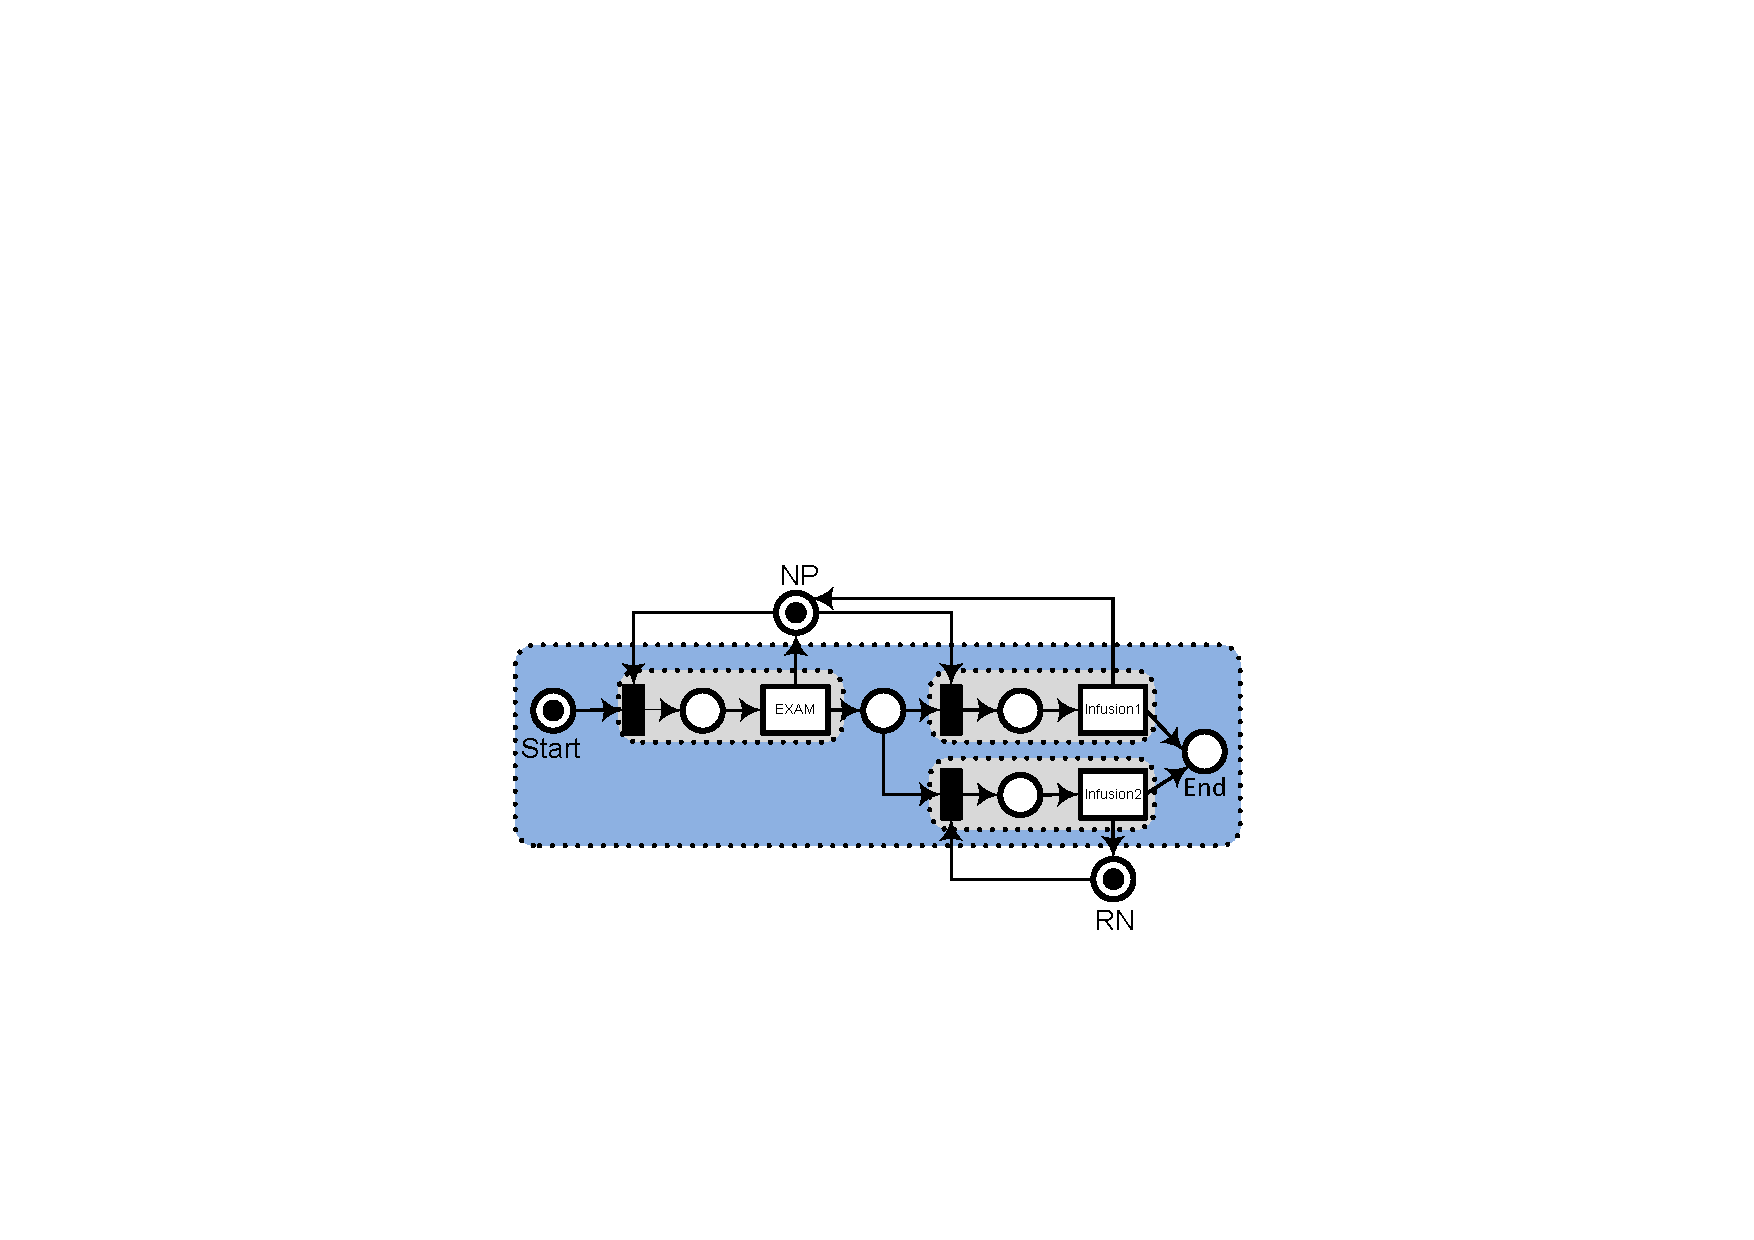
\includegraphics[scale=0.6]{SDNet.pdf}
	\caption{An SDRR Net of a Hospital Process.}
	\label{fig:sdr-net}  
	\vspace{-1em}
\end{figure}



Given an SDC, $\mathcal{S}$, we denote
$E_{\mathcal{S}}$ (and $E_{\mathcal{S}}'$), $P_{\mathcal{S}}$, $F_{\mathcal{S}}$ its
sets of transitions (and timed transitions), places and flows,  respectively.
Furthermore, the set of places that precede (follow) the immediate (timed) transition of $\mathcal{S}$ is denoted by 
$\bullet E_{\mathcal{S}}$ ($E_{\mathcal{S}} \bullet$), i.e., \begin{align*}
&\bullet E_{\mathcal{S}} = \{p \in P \ | \ \forall e \in E_{\mathcal{S}} \setminus E_{\mathcal{S}}': \ p \in \bullet e \} \\
&E_{\mathcal{S}} \bullet = \{p \in P \ | \ \forall e' \in E_{\mathcal{S}}' : \ p \in e'\bullet \}. \\
\end{align*}

Detecting the SDCs of a given TPN is linear in the number of transitions ($\mathcal{O}(|E|+|P|)$), since 
it involves traversing over the immediate transitions of the TPN and verifying
that the transition is followed by a single place,
which is in turn followed by 
a single timed transition (see Definition~\ref{def:sdc}).



A TPN that comprises a set of SDCs is referred to 
as a seize-delay-release net (SDR net). To define 
an SDR net, we let $S= \{\mathcal{S}_1,\ldots,\mathcal{S}_m\}$ be a set of SDCs.
The set $S$ can be partitioned into 
$k$ sets denoted by $C = \{\mathcal{C}_1,\ldots, \mathcal{C}_k\}$, 
with each set $\mathcal{C}_j, j = 1,\ldots, k$ containing 
SDCs that have equal 
input and output places. It is easy to show 
that $C$ always exists and that it is unique for 
a given TPN.
To simplify notation, we denote $E_{\mathcal{C}_j}$ ($E_{\mathcal{C}_j}'$)
the transitions (timed transitions)
of the SDCs that are elements of 
$\mathcal{C}_j$. We are now ready to define 
seize-delay-release nets.

\begin{mydef} [Seize-Delay-Release Net] \label{def:sdnet}
	A seize-delay-release net is a timed Petri net, 
	$\mathcal{N}_{sdr} = (E, E', P , F, \tau)$, which satisfies the following
	conditions:
	\begin{itemize}
		\item The set $\bigcup_{j=1}^{m} E_{\mathcal{S}_j}$ contains only transitions 
		from the set of SDCs ($E' \subseteq E$ being 
		the set of timed transitions), 
		\item The set $P = \bigcup_{j=1}^m P_{\mathcal{S}_j} \cup P_{c}$ contains 
		both the delay places
		of $N$ and a finite set of $k+1$ connector places $P_{c} = \{p_1,\ldots, p_{k+1}\}$
		with $p_1, p_{k+1} \in P_c$ being unique source and sink places, respectively, and, 
		\item The flow $F = \bigcup_{j=1}^m F_{\mathcal{S}_j} \cup F_c$ contains
		both the set of SDC
		flows and a set $F_c$ 
		such that \begin{align} \label{eq1}
		F_c = & \{(p,e) \in P_c \times E \setminus E' \ | \\ & p = p_j \ \land \exists\mathcal{C}_j \in C (\ e \in E_{\mathcal{C}_j} \setminus E_{\mathcal{C}_j}') \} \ \cup \nonumber\\
		&\{(e,p) \in E' \times P_c \ | \\ &\exists \mathcal{C}_j \in C (e \in E_{\mathcal{C}_j}' \ \land \ p = p_{j+1}) \}.
		\end{align}
	\end{itemize}
\end{mydef} An example for an SDR net can be found in Figure~\ref{fig:sdr-net}. The blue area corresponds to an SDR net that consists of three SDCs partitioned
into two sets, namely an SDC that involves `Exam' and two SDCs that correspond to Infusion 
(transitions Infusion1 and Infusion2 are 
part of the same set in the partition of SDCs, $C$). Furthermore,
the place of connectors $P_c$ contains three places: start place, 
end place and 
a place that connects `Exam' to the two `Infusion' SDCs.
SDR nets are important building blocks of the
Seize-Delay-Release nets with resources (SDRR nets),
which we map into basic scheduling problems. Algorithm~\ref{Alg1} verifies that a TPN
is an SDR net.



\begin{algorithm}[h!]
	
	\LinesNumbered
	\DontPrintSemicolon
	\SetAlgoLined
	\KwIn{Timed Petri net $\mathcal{N} = \langle E, E',P, F, \tau \rangle$}
	\KwOut{$\langle \{\mathcal{S}_1,\ldots,\mathcal{S}_m\}, P_c \rangle$ - Set of SDCs and set
		of connector places $P_c$}
	\Begin{
		
		
		$P_{in} \leftarrow \{p \in P \ | \ \bullet p = \emptyset\}$\;
		$P_{out} \leftarrow \{p \in P \ | \ p \bullet = \emptyset\}$\;
		\uIf{$|P_{in}| \neq 1 \ \lor |P_{out}| \neq 1 $}
		{\Return False \; }
		
		$S = \{\mathcal{S}_1,\ldots,\mathcal{S}_m\} \leftarrow$ \emph{DetectSDC}$(\mathcal{N})$\;
		
		\uIf{$\bigcup_{j=1}^{m} E_{\mathcal{S}_j} \neq E$}
		{\Return False \; }
		
		$C \leftarrow \{\mathcal{C} \subseteq S \ | \ \forall \mathcal{S}_i,\mathcal{S}_j \in \mathcal{C} :$ \ $ \bullet E_{\mathcal{S}_i} = \bullet E_{\mathcal{S}_j} \ \land \
		E_{\mathcal{S}_i} \bullet =  E_{\mathcal{S}_j} \bullet\}$\;
		
		
	
		\ForEach{$\mathcal{C}_j \in C$}{
		$\bullet\mathcal{C}_j = \bigcup_{\mathcal{S} \in \mathcal{C}_j} \bullet E_{\mathcal{S}}$\;
		$\mathcal{C}_j\bullet = \bigcup_{\mathcal{S} \in \mathcal{C}_j} E_{\mathcal{S}} \bullet$\;
		\uIf{$(\bullet\mathcal{C}_j =  \mathcal{C}_j\bullet \ \lor \ 
			|\bullet\mathcal{C}_j| \neq 1 \ \lor 
			\ |\mathcal{C}_j\bullet| \neq 1$}{\Return False \;}	
		
		}
		\uIf{$\exists \mathcal{C}_i \neq \mathcal{C}_j \in C \ (\mathcal{C}_i \bullet = \mathcal{C}_j \bullet 
		\ \lor \ \bullet\mathcal{C}_i  = \bullet\mathcal{C}_j)) $}{\Return False \;}	
	
		
		$P_c \leftarrow \bigcup_{\mathcal{C}_j \in C} (\bullet\mathcal{C}_j \cup  \mathcal{C}_j \bullet) $\;
		$F_c \leftarrow \bigcup_{\mathcal{C}_j \in C} \{(x,y) \in F \ | \  (x \in \bullet\mathcal{C}_j \ \land \ y \in E_{\mathcal{C}_j} \setminus E_{\mathcal{C}_j}' ) \ \lor \ (x \in E_{\mathcal{C}_j}' \ \land \ y \in \mathcal{C}_i \bullet)\}$\;

		
		\uIf{$P_c \neq P \setminus \bigcup_{j=1}^{m} P_{\mathcal{S}_j} \ \lor \ F_c \neq F \setminus \bigcup_{j=1}^{m} F_{\mathcal{S}_j}$}
		{\Return False \; }
		\Return True \;
	}
	
	
	\caption{Verifies that TPN is SDR net.}
	\label{Alg1}
\end{algorithm}

\todo{update explanation and proof}
  


Below, we explain the algorithm line-by-line. Lines 2-5
verify that the TPN has unique input and output places. Line 6 
returns the set of SDCs, $S$, that 
are present in 
the input TPN. 
Detecting SDCs is performed via the function \emph{DetectSDC}$(\cdot)$,
which uses a simple traversal over all immediate transitions 
$e \in E \setminus E'$ and checking whether the direct followers of $e$ are 
a single place and a timed transition (as in Definition~\ref{def:sdc}). 
Lines 7-8 make sure that the set of transitions $E$ includes
only transitions from $S$. 

Line 9 partitions 
the SDCs into sets of SDCs, such that
each set $\mathcal{C} \in C$ contains only 
SDCs that share input and output places. 

Lines 10-15 traverse the sets in $C$ and 
verify that each set $\mathcal{C}_j \in C$ has a unique input 
place and a unique output place 
($|\bullet\mathcal{C}_j| = |\mathcal{C}_j\bullet| =1$). 
Furthermore, Lines 10-13
ensure that the input and output places of $\mathcal{C}_j$
are not equal to each other (no loops), and that 
there does not exist an additional set $\mathcal{C}_i \neq \mathcal{C}_j$
for which one of its input or output places are equal to 
the corresponding input and output places of $\mathcal{C}_j$. 
Intuitively, this enforces a sequential execution of the sets 
of SDCs in $C$. Lines 14-17 check whether the TPN places
can be either SDC places or connectors ($P_c$)
and that the only flows allowed in the TPN 
are within SDCs or between connector places, $P_c$, 
and SDC constructs.

If the algorithm reaches Line 18 without breaking,
it concludes that the TPN is an SDR net and returns its set of SDCs $S$ and
the set of connector places $P_c$. Proposition~\ref{prop:corrAlg1} states the 
correctness and completeness of Algorithm~\ref{Alg1}.
\todo{polish proof}

\begin{myprop} \label{prop:corrAlg1}
	Algorithm~\ref{Alg1} is correct and complete, 
	i.e., the algorithm returns non-empty sets, if and only if, the input TPN
	is an SDR net. 
\end{myprop}
\begin{proof} \noindent \emph{If: Given an input TPN that is an SDR net, the algorithm returns non-empty sets.}\\
	The input TPN is an SDR net. Hence, by Definition~\ref{def:sdnet}, it has a source and a sink. Furthermore, $E = \bigcup_{j=1}^m E_{\mathcal{S}_j}$
	and therefore Lines 4 and 7 return True. 
	In an SDR net, all flows are either 
	in $\bigcup_{j=1}^m F_{\mathcal{S}_j}$ (being part of an SDC) 
	or in $F_c$, i.e., connecting places in $P_c = \{p_1,\ldots, p_{k+1}\}$
	to the set of SDCs in the partition set, $C$. Furthermore, from the definition of $F_c$ 
	each partition set $\mathcal{C}_j$ has exactly a single direct predecessor place $p_j \in P_c$
	and a single direct successor place $p_{j+1}$. Moreover, no two 
	sets in $C$ can have the exact same predecessors and successors (otherwise, they would 
	not be two different sets in $C$). Therefore, the condition in Line 13
	holds for every $\mathcal{C}_j \in C$.\\	
		
	\noindent \emph{and only If: 
	Given that the algorithm returns non-empty sets, the input net is an SDR net.}\\
	We prove the second direction by using the intermediate 
	computations
	of Algorithm~\ref{Alg1} to construct an SDR net $\mathcal{N} = (E, E',P, F, \tau)$
	and showing that the net $\mathcal{N}$ is equal to the input TPN. 
	
	
		

	
\end{proof}


Having defined SDR nets and an algorithm that verifies whether 
a given TPN is an SDR net, we
define the seize-delay-release net with resources (SDRR net),
which is a timed Petri net that consists of a set of SDR nets and a set of places
and flows that correspond to resources. Let $N_{sdr} = \{\mathcal{N}_1,\ldots,\mathcal{N}_n\}$ be a set of 
SDR nets with $\mathcal{N}_j = \langle E_j, E'_j , P_j , F_j, \tau_j\rangle, j = 1, \ldots, n$ and
let $S = \{\mathcal{S}_1,\ldots,\mathcal{S}_m\}$ be a set of SD constructs
that participate in $N_{sdr}$. We are now ready to define the SDRR nets. 

\begin{mydef} [Seize-Delay-Release Net with Resources (SDRR net)] \label{def:sdr-net}
	An SDR net with resources (SDRR net) is a timed Petri net, 
	$\mathcal{N}_{sdrr} = (E, E', P , F, \tau)$, such that 
	\begin{itemize}
		\item The set \small $E = \bigcup_{j=1}^n E_j$ contains only transitions from the SDNs ($E' \subseteq E$ being 
		the set of timed transitions), 
		\item The set \small $P = \bigcup_{j=1}^m P_j \cup P_{r}$ contains both places from $N$ 
		and a finite set of resource places $P_{r}$, and, 
		\item The flow set \small $F = \bigcup_{i=1}^m F_i \cup F_r$ contains		
		all SDN 
		flows and a set $F_r$ 
		such that:  
		\small
		\begin{align*}
		F_r = &\{ (x,y) \in (P_r \times E \setminus E') \cup
		(E' \times P_r) \ | \ \forall (x,y) \in F_r: \\  &Q(x,y,S) \}
		\end{align*}
		with, \small \begin{align*} &Q(x,y,S) =\\ 
		&((x \in P_r \land y \in E_{\mathcal{S}_i} \setminus E_{\mathcal{S}_i}'  \Rightarrow \exists (e',x) \in F_r: \ e' \in E_{\mathcal{S}_i}') \\
		& \land \ (x \in E_{\mathcal{S}_i}' \land y \in P_r \Rightarrow \exists (y,e) \in F_r: \ e \in E_{\mathcal{S}_i} \setminus E_{\mathcal{S}_i}').\end{align*}
	\end{itemize}
\end{mydef} The set of resource flows $F_r$ allows for resource tokens to be consumed only by immediate transitions and produced 
only by timed transitions. Furthermore, the property $Q(x,y)$ makes sure that 
if an immediate 
transition that consumes a resource token 
is part of an SDC, say $\mathcal{S}_i$, then there must 
also be a flow between the timed transition of $\mathcal{S}_i$ back
to the same resource place. Similarly, if a timed transition of an SDC produces a resource 
token, there must be a flow between the resource 
place and the immediate transition of the same SDC.
One
can easily verify that Figure~\ref{fig:sdr-net} 
is an SDRR net with a single SDR net, three SDCs and two resource places 
($NP$ for nurse practitioner and $RN$ for registered nurse). 


Next, we introduce Algorithm~\ref{Alg2},
which  
take a TPN as its input, and returns
whether the TPN is an SDRR net. 


\begin{algorithm}[h!]
	
	\LinesNumbered
	\DontPrintSemicolon
	\SetAlgoLined
	\KwIn{Timed Petri net $\mathcal{N} = \langle E, E',P, F, \tau \rangle$}
	\KwOut{True or False}
	\Begin{
		
		%\tcc{Step 1: Find resource places by removing}
		$S = \{\mathcal{S}_1,\ldots,\mathcal{S}_m\} \leftarrow$ \emph{DetectSDC}$(\mathcal{N})$\;
		$P_r \leftarrow \{p \in P \ | \ \forall (x,y) \in F_{\{p\}} ( Q(x,y,S))  \}$\;
		$\mathcal{N}' =(E, E',P \setminus P_r, F \setminus F_{P_r}, \tau)$\; 
		$\{\mathcal{N}_i\}_{i=1}^{n} \leftarrow$ \emph{ConnectedComponents}$(\mathcal{N}')$\;
		\uIf{$\exists i \in [n] :$ \emph{VerifySDR}$(\mathcal{N}_i) $ = False}
		{\Return False\;}

		\Return True\;
	}


	\caption{Verifies that TPN is SDR net with resources (SDRR net).}
	\label{Alg2}
\end{algorithm}

\todo{update this part for the new algorithm}
We shall briefly go over the algorithm and 
explain its parts. Lines 2-7 serve us to identify 
a set of places $P_r$ that are candidates to be
the resource places of the resulting SDRR. 
In an SDRR,
a necessary condition for every $p \in P_r$ is 
that when $p$ is removed from the net (along
with the incoming and outgoing flows $F_{\{p\}}$) 
there will still exist a path between SDR net sources 
to their corresponding sinks. Removing a non-resource place,
i.e., a place from one of the SDR nets of the SDRR net, 
will result in a source without a path to its sink. 
Therefore, removing places from the input TPN
and verifying that every source has a path to a sink (via the
function \emph{AllSourceToSink} that receives a TPN and checks whether 
every source has a path to a sink),
enables us to find candidates for $P_r$. 
Then, in Line 8, we remove all places in $P_r$ from the input TPN
and store the resulting net $\mathcal{N}'$. In Line 9,
we store the connected components of $\mathcal{N}'$ in a set of
TPNs $\{\mathcal{N}_i\}_{i=1}^{n}$. If the input is an SDRR, 
this set will contain $n$ SDR nets. Therefore, in Lines 12-18,
we verify that the $n$ connected components are SDR nets. 
Verifying whether $\mathcal{N}_i$ is an SDR net 
is performed by running a 
Breadth-First Search (BFS) algorithm that 
verifies the conditions in Definition~\ref{def:sdnet}.
The procedure \emph{VerifySDR}$(\cdot)$ returns $\emptyset$
if $\mathcal{N}_i$ is not an SDR (which will lead to 
an answer False in Algorithm~\ref{Alg2} due to a violation of Definition~\ref{def:sdr-net});
otherwise,
it returns the set $P_{c,i}$, which is the connector set of the
now verified SDR net $\mathcal{N}_i$, and $S_i$,
which is the set of SDCs that $\mathcal{N}_i$ comprises.
Lastly, Lines 19-20 check whether the set of 
candidate resource places, $P_r$, satisfies $Q(x,y,S)$ 
from Definition~\ref{def:sdr-net}. If one of the flows
into $p \in P_r$ violates $Q(x,y,S)$, the algorithm returns False.
Otherwise, the algorithm returns True.


 \todo{polish proof}
\begin{myprop} \label{prop:corrAlg2}
	Algorithm~\ref{Alg2} is correct and complete, 
	i.e., the algorithm returns \emph{True}, if and only if, the input to the algorithm
	is an SDRR net. 
\end{myprop}
\begin{proof} \noindent \emph{If: Given an input TPN that is an SDRR net, the algorithm returns True.}\\
If $\mathcal{N}$ is an SDRR net, then the only places that would not interrupt the flow between every source 
and sink of its SDR nets in $N_{sdr}$, are places in $P_r$. 
Therefore, the set $P_r$ computed by the algorithm will contain only resource places
of the SDRR net. 
After removing the resource places and their corresponding flows (Line 8),
we are remained with $n$ connected components, with each component being an SDR net (Line 9).
The algorithm will verify the following two conditions: (1) the $n$ components are SDR nets (Lines 10-18),
and (2) the set of flows $F_r$ respects $Q(x,y,S)$ (since the TPN is an SDRR net). Therefore it will return 
True.\\

	
	
\noindent \emph{and only If: Given that the algorithm returns True, the input net is an SDRR net.}\\
We prove the second direction by using the intermediate 
computations
of Algorithm~\ref{Alg1} to construct a Petri net $\mathcal{N} = (E, E',P, F, \tau)$
and showing that $\mathcal{N}$ corresponds to an SDRR net (Definition~\ref{def:sdr-net}). We
compose the SDRR net by 
connecting the TPNs $\mathcal{N}_i, i = 1, \ldots, n$ (which are verified to be SDR nets by Lines 10-18) to the set of places
$P_r$ using the flow set $F_r$. Since the flows $F_r$ respect property $Q(x,y)$, 
the resulting net is an SDRR net according to Definition~\ref{def:sdr-net}.

\end{proof}




\section{Transforming SDPN to CP Models}
\label{TPN2CP}

In this part, we present a
transformation of schedule-driven Petri nets (SDPNs)
to constraint programming (CP) formulations. To this end, we define
the \emph{basic scheduling constructs set} (BSCS). Subsequently,
we show that the BSCS can be derived from the SDPN. Lastly, we
construct CP models from a given BSCS, thus completing the TPN2CP phase of our solution.  

\subsection{The Basic Scheduling Constructs Set}
The BSCS will contain the activities to be scheduled, the resources
along with their capacities, precedence constraints, and 
activity-and-resource dependent durations. In essence, the BSCS contains a set of building blocks of  
many well-known scheduling 
problems such as the 
job-shop scheduling problem (JSSP), 
and the resource-constrained project scheduling problem (RCPSP) 
(including its multi-mode variation). To define BSCS,
we follow the scheduling problem 
definition introduced by~\cite{van1996petri}.

\begin{mydef} [Basic Scheduling Constructs Set BSCS)] \label{def:sched}
Basic scheduling constructs are a set $B = \{ \mathcal{A}, \mathcal{R}, \varPi, c, d \}$ over a 
	over a finite time domain $\mathcal{T}$
	with,
	\begin{itemize}
		
		\item $\mathcal{A}$ being the set of activities to be scheduled,
		\item $\mathcal{R}$ being the set of renewable resources,
		\item $\varPi \subseteq \mathcal{A} \times \mathcal{A}$ being the precedence relation between pairs of activities,
		\item $c: \mathcal{R} \rightarrow  \mathbb{N}^{+}$ being the function that maps resources to their capacities, and, 
		\item $d: \mathcal{A} \times 2^{\mathcal{R}} \nrightarrow \mathcal{T}$ being the duration partial function that maps pairs of activities and resource sets (that can execute these activities) to values in the time domain.
		%	and, \item $b: \mathcal{A} \times 2^{\mathcal{R}} \times \mathcal{R} \nrightarrow \mathbb{N}^{+}$ being the demand partial function for resources when 
		%	executing an activity by a specific resource set. \todo{requires the addition of weights on the TPN!!}
	\end{itemize}
\end{mydef} \noindent A schedule $s$, which satisfies
a BSCS, is an allocation of resource sets to 
activities over time, i.e., 
$s \in \mathcal{A} \rightarrow  (2^\mathcal{R} \times \mathcal{T})$. A feasible schedule respects 
resource and precedence constraints. 
Without loss of generality, one often considers an objective function 
$\phi(s) \in \mathcal{R}^{+0}$ that 
assigns a real-valued number to a 
given schedule. In optimal scheduling one aims at finding a 
schedule that minimizes 
$\phi(s)$. In this work, we avoid learning
the objective function of the underlying scheduling problem, and hence assume that $\phi$ is given.

A prominent example that can be constructed using the BSCS is the \emph{job shop scheduling problem} (JSSP),
where only a single resource can perform each activity (hence $d(a) , a \in \mathcal{A}$ is sufficient to represent durations),
and resource capacities are equal to $1$. The objective function in
JSSP is to minimize the makespan.

\subsection{Deriving BSCS from SDPN}

In this part, we provide a 
mapping from Seize-Delay-Release 
timed Petri nets with resources (SDRR nets) into 
basic scheduling problems (BSPs). Specifically, 
given an SDRR net, $\mathcal{N} = \langle E, E',P, F, \tau \rangle$, our
we propose a mapping  that creates the corresponding BSP tuple, $\langle  \mathcal{A}, \mathcal{R},\varPi, c, d \rangle$.

For conciseness, 
we refer to elements of the TPN 
(e.g., places, transitions, flows)
when defining the BSP instead of labeling the TPN
and then using these labels to define the BSP. \todo{not sure that this needs to be said here}

For an SDRR net, we may reuse parts of
Algorithms~\ref{Alg1} and~\ref{Alg2} to derive the following
sets: (1) the set of SDCs $S = \{\mathcal{S}_1,\ldots,\mathcal{S}_m\}$,
(2) the set of resource places $P_r$, (3) 
the set of SDR nets that comprise the 
SDRR net $N_{sdr} = \{\mathcal{N}_i\}_{i=1}^{n}$ (4) the set of 
connector places $P_c = \{P_{c,i}\}_{i=1}^{n}$ for every SDR net
that comprises the SDRR net, and (5) the 
partition of SDCs, $\{C_i\}_{i=1}^{n}$, 
which includes sets of SDCs with common 
input and output connectors in the $i$th SDR net. 

\begin{mydef}[SDRR net to BSP Mapping]
	\begin{sloppypar} Given an SDRR net $(\mathcal{N} = (E, E', P, F, \tau), m_0)$ 
		and the sets $S, P_r,  N_{sdr}, P_{c,i}, C_i$,
		the BSP is constructed as follows:\end{sloppypar}
	\begin{itemize}
		\item The resource set is 
		given by the set of places, $\mathcal{R} = P_r$,
		\item The activity set corresponds to all connector places in $P_c$ except the sinks, namely $\mathcal{A} = \{p \in P_c | p\bullet \neq \emptyset \}$,
		\item The precedence
		relation $\varPi$ is constructed using
		the following: $$\varPi = \{(a,b) \in \mathcal{A} \times \mathcal{A} \ | \ a \rightsquigarrow b\},$$
		with $\rightsquigarrow$ indicating that there exists a path from $a$ to $b$,
		\item resource capacities, $c$, are equal to the
		initial marking
		of resource places, i.e., $\forall r \in \mathcal{R}: c(r) = m_0(p_r)$, and finally, 
		\item the duration (partial) function $d$ is computed as follows:
		\begin{align*} d = & \{ (a,R,d) \in \mathcal{A} \times 2^{\mathcal{R}} \times \mathcal{T} \ | \\
		& \forall \mathcal{S} \in S (\forall e \in E_{\mathcal{S}} \setminus E_{\mathcal{S}}'( a \in \bullet e  \ \land 
		\ R \subseteq (\bullet e \cap \mathcal{R})) \\ &\land \forall e' \in   E_{\mathcal{S}}' (d = \tau(e')) ) \} 
		\end{align*}	
	\end{itemize} 
\end{mydef}


\subsection{From BSCS to CP Models}
\todo{Kyle, please insert BSP to CP here. Chris will add a part on the intuition for scheduling people}




\section{Evaluation}
\label{sec:evaluation}



\section{Related Work}
\label{sec:relwork}

\section{Conclusion}
\label{sec:conclusion}

\bibliographystyle{aaai}
\bibliography{Biblio}


%\appendix{Algorithms}
%
%
%
%
%
%
%
%
%
%\begin{algorithm}[t!]
%	
%	\LinesNumbered
%	\DontPrintSemicolon
%	\SetAlgoLined
%	\KwIn{SDR-TPN $(\mathcal{N} = (E, E', P, F, \tau), m_0)$, SDR decomposition 
%		$D_{sdr}((\mathcal{N}, m_0)) = \{(\mathcal{N}_1, m_0^1), \ldots, (\mathcal{N}_n, m_0^{n-2}) , (\mathcal{N}_r, m_0^{r}), (\mathcal{N}_j, m_0^{j})\}$, $P_a$, $P_r$.}
%	\KwOut{Set of activities and precedence order, $\mathcal{A}, \varPi$.}
%	\Begin{
%		
%		\tcc{Find activities from sets of SD constructs with
%			joint input place. Every input place 
%			into an SD construct corresponds to one activity.}
%		$\mathcal{A} = \{p \in P \ | \ \exists \ e \in E \setminus E'(p \in \bullet e) \}$;\\
%		\tcc{Create a new without resource places and flows between resources places and 
%			SD constructs. The function $Follows(G, a, a')$ returns True if
%			there is a path from $a$ to $a'$ in a directed graph $G$.}
%		$F_r = \{(x,y) \in F | x\in P_r \lor y \in P_r  \}$;\\
%		$\mathcal{N}'= (E, E', P \setminus P_r, F \setminus F_r, \tau), m_0)$;\\
%		$\varPi = \{(a,a') \in \mathcal{A} \times \mathcal{A} \ | \ Follows(\mathcal{G}(\mathcal{N}'), a, a')  =True$ \};\\
%		\Return $\mathcal{A}, \varPi$;\\
%		
%	}
%	\caption{Constructs activity set $\mathcal{A}$ and precedence relation $\varPi$.}
%	\label{ConstructActPrec}
%\end{algorithm}
%
%
%
%
%
%
%\begin{algorithm}[t!]
%	
%	\LinesNumbered
%	\DontPrintSemicolon
%	\SetAlgoLined
%	\KwIn{SDR-TPN $(\mathcal{N} = (E, E', P, F, \tau), m_0)$, SDR decomposition 
%		$D_{sdr}((\mathcal{N}, m_0)) = \{(\mathcal{N}_1, m_0^1), \ldots, (\mathcal{N}_n, m_0^{n-2}) , (\mathcal{N}_r, m_0^{r}), (\mathcal{N}_j, m_0^{j})\}$, $P_a$, $P_r$, set of activities $\mathcal{A}$, 
%		set of resources $\mathcal{R}$.}
%	\KwOut{Function $\rho$ and partial functions $d,b$.}
%	\Begin{
%		
%		\tcc{Go over the activities, and check which of the resources is connected, per execution mode.}
%		\For{$e \in E \setminus E'$}{$R(e) = \{r \in P_r \ | \ (r,e) \in F  \}$;\\}
%		\For{$a \in \mathcal{A}$}{$\rho(a) = \{ R(e) \ | \ (a,e) \in F \}$;\\}
%		\tcc{Retrieve the SD net that corresponds to a combination of $a$ and $R$.}
%		
%		
%		
%		\For{$a \in A$}{
%			\For{$R \in \rho(a)$}{
%				$i(a,R) = \forall i \in I^n(\exists e \in E_i((a,e) \in F))$;\\
%				$d(a, R) = \{ \tau(e') \ | \ e' \in E'_{i(a,R)}  \}$;\\}}
%		
%		\Return $\rho, d, b$;\\	
%	}
%	
%	\caption{Constructs: RTAA function, duration partial function, and demand partial function.}
%	\label{ConstructRhoDur}
%\end{algorithm}
%
%




%\balance
%\newpage




\end{document}


